\documentclass[a4paper,11pt]{article}

% Configuración de página
\usepackage{geometry}
\geometry{left=10mm, right  =25mm, top=35mm, bottom=30mm, headheight=35mm}

% Paquete para justificar el texto
\usepackage{ragged2e}

% Referencias
\usepackage{hyperref} % Para hacer hipervínculos
\usepackage{colorlinks=true,linkcolor=blue} % Para que aprezca de color rojo por defecto los hipervínculos


% Paquete de idioma
\usepackage[spanish, es-nodecimaldot, mexico]{babel} % mexico es para que aparezca en laa leyenda de tablas y no cuadros en las tablas.

\usepackage[utf8]{inputenc}

%Fecha
\usepackage[useregional]{datetime2}

% Paquetes de fuentes
\usepackage{courierten}
\renewcommand*\familydefault{\ttdefault} %% Only if the base font of the document is to be typewriter style
\usepackage[T1]{fontenc}

% Paquetes de colores
\usepackage[table]{xcolor} % Table es para utilizar los colores en tablas también.
\definecolor{colorRojo1}{rgb}{1.0, 0.03, 0.0}
\definecolor{colorAzul1}{rgb}{0.0, 0.75, 1.0}
\definecolor{colorGris1}{rgb}{0.75, 0.75, 0.75}
\definecolor{colorGris2}{rgb}{0.66, 0.66, 0.66}


% Encabezados
\usepackage{lastpage}
\usepackage{fancyhdr}
\pagestyle{fancy}

\color{colorGris1}\renewcommand{\headrulewidth}{0.5mm}
\renewcommand{\footrulewidth}{0.2mm}

% Pie de página
\lfoot{\small Notas sobre LaTeX}
\cfoot{}
\rfoot{\small Página. \thepage\ / \pageref{LastPage}}

% Encabezado
\lhead{LUCHO}
\chead{\autor}
\rhead{\DTMsetstyle{ddmmyyyy}\fecha}

% Paquetes de figuras
\usepackage{graphicx} % Carga las figuras
\graphicspath{{./Figuras}} % Indica la dirección de las figuras
\usepackage{float} % Permite poner la posición H
\usepackage{subcaption} % Permite poner subfiguras
\usepackage{wrapfig} % Para envolver el texto alrededor de la figura
\usepackage{overpic} % Para poner texto sobre las figuras

% Paquete de tablas
\usepackage{booktabs} % Para darle varios tipos de líneas en las tablas
\usepackage{colortbl} % Para darle color a las tablas

\begin{document}
	\noindent
	% Comandos personalizados
	\newcommand{\fecha}{\DTMdate{2024-02-25}}
	\newcommand{\titulo}{NOTAS SOBRE LATEX}
	\newcommand{\autor}{Luis ZG}
	
	\begin{center}
		\color{colorRojo1} \LARGE \textbf{\titulo} \vspace{5mm}
		
		\color{colorAzul1} \textbf{Manual de ayuda}
		
		\color{colorAzul1} \underline {Por: \autor.}
	\end{center}
	
	\begin{flushright} \color{colorGris1}
		Inicio: Domingo 25 de febrero del 2022
		
		Fin: \fecha
	\end{flushright}
	
	\newpage
	
	\color{colorAzul1} \tableofcontents
	
	\clearpage
	
	\begin{flushleft} \color{colorGris2}
		
		\section{Comandos rápidos}
		
		Ctrl + flechaDerecha: Cambia de opción en el editor TeXstudio.\newline
		
		Ctrl + clic: Lleva a la palabra que pertenece entre editor y el PDF.\newline
		
		\textbackslash indent: Inserta sangría.\newline
		
		\textbackslash noindent: Elimina sangría.\newline
		
		\textbackslash textbackslash: Inserta el carácter \textbackslash.\newline
		
		\textbackslash \%: Inserta el símbolo de porcentaje.\newline
		
		\textbackslash \$: Inserta el símbolo del dólar.\newline
		
		\textbackslash \#: Inserta el símbolo del numeral.\newline
		
		\textbackslash \&: Inserta el símbolo del and.\newline
		
		\textbackslash \_: Inserta el símbolo sub guion.\newline
		
		\section{Configuración del documento}
		
		Comando: \textbackslash documentclass[a4paper, 11pt]\{article\}\newline
			
		Acción: Configura el documento  a formato de hoja A4, con tamaño de texto 11pt en tipo de documento artículo.\newline
			
		\section{Entorno del documento}
			
		Comando: \textbackslash begin\{document\}\newline
		Aquí van los párrafos del documento.\newline
		\textbackslash end\{document\}\newline
			
		Acción: Todos los entorno empieza con Begin y terminan con end y el nombre del entorno entre corchetes.\newline
		
		\section{Paquete de colores}
		
		Comando: \textbackslash usepackage\{xcolor\}\newline
		\textbackslash definecolor\{rojo1\}\{rgb\}\{1.0, 0.03, 0.0\}\newline
		\textbackslash definecolor\{azul1\}\{rgb\}\{0.0, 0.75, 1.0\}\newline
		\textbackslash definecolor\{gris1\}\{rgb\}\{0.75, 0.75, 0.75\}\newline
		\textbackslash definecolor\{gris2\}\{rgb\}\{0.66, 0.66, 0.66\}\newline
			
		Acción: Sirve para configurar los colores que se utilizará en el documento.\newline
		
		\section{Paquete de fuentes}
			
		Comando: \textbackslash renewcommand*\textbackslash ttdefault\{lcmtt\}\newline
		\textbackslash renewcommand*\textbackslash familydefault\{\textbackslash ttdefault\}\newline
		\textbackslash usepackage[OT1]\{fontenc\}\newline
			
		Acción: Sirve para personalizar las fuentes del documento.\newline
		
		\section{Paquete de idioma}
			
		Comando: \textbackslash usepackage[spanish, es-nodecimaldot]\{babel\}\newline
		\textbackslash usepackage[utf8]\{inputenc\}\newline
			
		Acción: Sirve para indicarle a TeXstudio que estamos trabajando en el idioma español con la configuración utf8, el paquete de idiomas se llama babel, el parámetro es-nodecimaldot es para que el separador de decimales sea el punto y no  la coma.\newline
		
		\section{Secciones}
		
		Comando: \textbackslash section\{nombre de la sección\}\newline
		
		Acción: Sirve para generar secciones numeradas, si se desea que no  se vea el número, el comando  sería \textbackslash section*\{Secciones\} tener cuidado no ponerle asterisco a la primera sección.\newline
		
		\section{Índice}
		
		Comando: \textbackslash tableofcontents\newline
		
		Acción: Sirve para generar el índice, para actualizar el índice se debe compilar 2 veces.\newline
		
		\section{Salto de página}
		
		\subsection{Comando 1:} \textbackslash newpage\newline
		\subsection{Comando 2:} \textbackslash clearpage\newline
		
		Acción: Sirve para hacer saltos de páginas y para figuras y elementos flotantes se recomienda clearpage.\newline
		
		\section{Listas no numeradas}
		
		Comando: \textbackslash begin\{itemize\}\newline
		\textbackslash item hola1\newline
		\textbackslash item hola2\newline
		\textbackslash end\{itemize\}\newline
		
		Acción: Sirve para generar listas no numeradas, si se desea una sub lista se hace lo mismo de la lista y si se desea cambiar el símbolo del inicio de las líneas de las listas en los ítem sepone paréntesis así: \textbackslash item[-].\newline
		
		\section{Listas numeradas}
		
		Comando: \textbackslash begin\{enumerate\}\newline
		\textbackslash item hola1\newline
		\textbackslash item hola2\newline
		\textbackslash end\{enumerate\}\newline
		
		Acción: Sirve para generar listas enumeradas.\newline
		
		\section{Listas con descripción}
		
		Comando: \textbackslash begin\{description\}\newline
		\textbackslash item[Descripción 1] Esta es la descripción 1.\newline
		\textbackslash item[Descripción 2] Esta es la descripción 2.\newline
		\textbackslash end\{description\}\newline
		
		Acción: Sirve para generar listas con descripciones y estas generan sangrias si el texto es muy extenso.\newline
		
		\section{Figuras}
		
		Comando: \textbackslash usepackage\{graphicx\}\newline
		\textbackslash graphicspath\{\{./Figuras\}\}\newline
		
		Acción: graphicx sirve para cargar las figuras y graphicspath sirve para indicar la dirección de las figuras.\newline
		
		\begin{figure}[h]
			\centering
			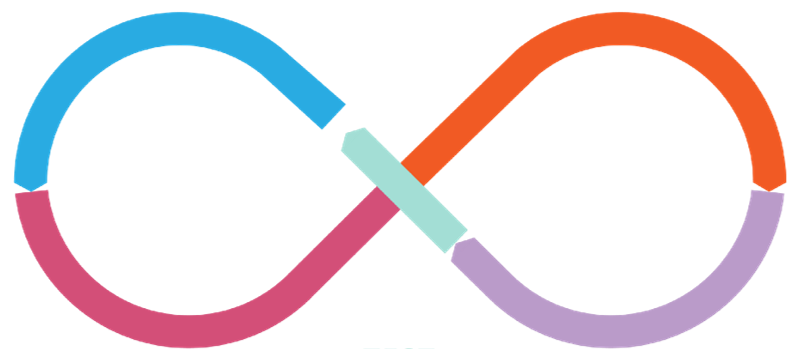
\includegraphics[width=0.25\textwidth]{flujo}
			\caption{Representación del infinito}
			\label{fig:flujo1}
		\end{figure}
		
		\begin{minipage}{0.99\textwidth}
			
			sfsdafa sagdgdf ggfdg gdfg gd gfdg gfgsgf ggsfg ggsdfg jhgjghjhk kjhgkhgkhg khgkhgkgh kjhkhkggkh khgkhgkh vxcvx cvxcv xcbcbvc bvcbv cbcvvnv nbmbn mnbmn bmn bmnb nbmnbmnb mn mnb mnbmbnmnb.
			
			\begin{wrapfigure}{l}{0.25\textwidth}
				\centering
				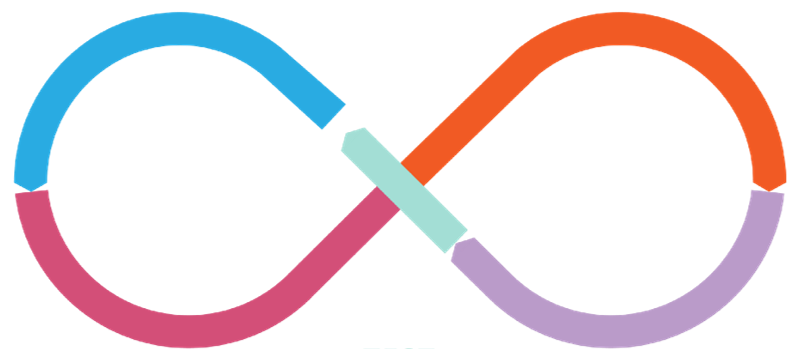
\includegraphics[width=0.9\linewidth]{flujo}
				\caption{Representación del infinito}
				\label{fig:flujo2}
			\end{wrapfigure}
			
			ggfdg gdfg gd gfdg gfgsgf ggsfg ggsdfg jhgjghjhk kjhgkhgkhg khgkhgkgh kjhkhkggkh khgkhgkh vxcvx cvxcv xcbcbvc bvcbv cbcvvnv nbmbn mnbmn bmn bmnb nbmnbmnb mn mnb mnbmbnmnb.
			
			sfsdafa sagdgdf ggfdg gdfg gd gfdg gfgsgf ggsfg ggsdfg jhgjghjhk kjhgkhgkhg khgkhgkgh kjhkhkggkh khgkhgkh vxcvx cvxcv xcbcbvc bvcbv cbcvvnv nbmbn mnbmn bmn bmnb nbmnbmnb mn mnb mnbmbnmnb.
			
			\begin{wrapfigure}{r}{0.25\textwidth}
				\centering
				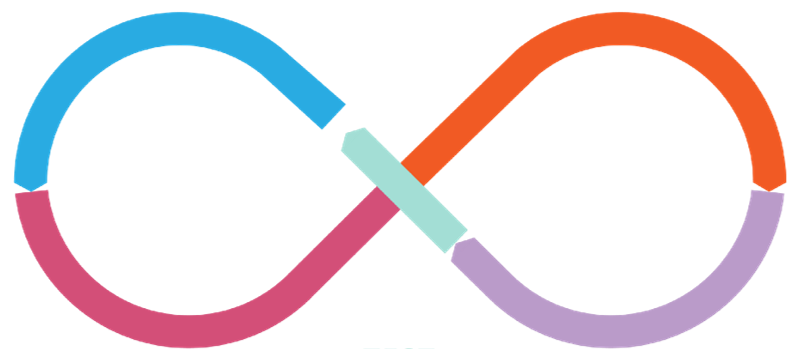
\includegraphics[width=0.9\linewidth]{flujo}
				\caption{Representación del infinito}
				\label{fig:flujo3}
			\end{wrapfigure}
			
			sfsdafa sagdgdf ggfdg gdfg gd gfdg gfgsgf ggsfg ggsdfg jhgjghjhk kjhgkhgkhg khgkhgkgh kjhkhkggkh khgkhgkh vxcvx cvxcv xcbcbvc bvcbv cbcvvnv nbmbn mnbmn bmn bmnb nbmnbmnb mn mnb mnbmbnmnb.
			
			dgdfgd gdffg sfdgfdgdfg gdfgdf
			
			ggfdg gdfg gd gfdg gfgsgf ggsfg ggsdfg jhgjghjhk kjhgkhgkhg khgkhgkgh kjhkhkggkh khgkhgkh vxcvx cvxcv xcbcbvc bvcbv cbcvvnv nbmbn mnbmn bmn bmnb nbmnbmnb mn mnb mnbmbnmnb.
			
			sfsdafa sagdgdf ggfdg gdfg gd gfdg gfgsgf ggsfg ggsdfg jhgjghjhk kjhgkhgkhg khgkhgkgh kjhkhkggkh khgkhgkh vxcvx cvxcv xcbcbvc bvcbv cbcvvnv nbmbn mnbmn bmn bmnb nbmnbmnb mn mnb mnbmbnmnb.
		\end{minipage}
		
		
		\section{Figuras que flotan}
		Ver en la imagen figura \ref{fig:flujo4}.
		\begin{figure}[H]
			\centering
			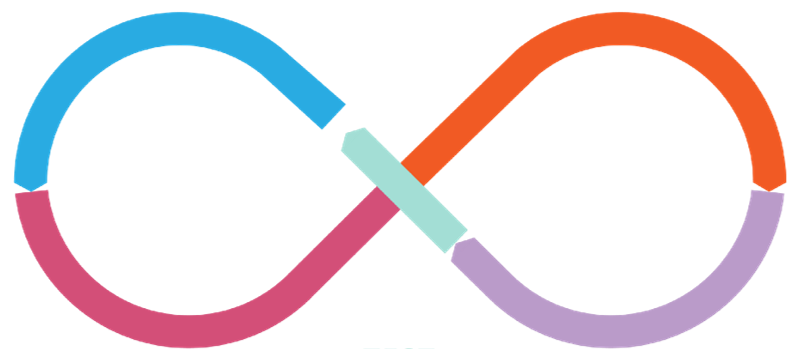
\includegraphics[width=0.6\linewidth]{flujo}
			\caption{Imagen sobre el infinito}
			\label{fig:flujo4}
		\end{figure}
		ggfdg gdfg gd gfdg gfgsgf ggsfg ggsdfg jhgjghjhk kjhgkhgkhg khgkhgkgh kjhkhkggkh khgkhgkh vxcvx cvxcv xcbcbvc bvcbv cbcvvnv nbmbn mnbmn bmn bmnb nbmnbmnb mn mnb mnbmbnmnb.
		
		
		\section{Dos figuras}
		ggfdg gdfg gd gfdg gfgsgf ggsfg ggsdfg jhgjghjhk kjhgkhgkhg khgkhgkgh kjhkhkggkh khgkhgkh vxcvx cvxcv xcbcbvc bvcbv cbcvvnv nbmbn mnbmn bmn bmnb nbmnbmnb mn mnb mnbmbnmnb.
		ggfdg gdfg gd gfdg gfgsgf ggsfg ggsdfg jhgjghjhk kjhgkhgkhg khgkhgkgh kjhkhkggkh khgkhgkh vxcvx cvxcv xcbcbvc bvcbv cbcvvnv nbmbn mnbmn bmn bmnb nbmnbmnb mn mnb mnbmbnmnb.
		
		\begin{figure}[h]
			\centering
			
\includegraphics[width=0.2\linewidth]{grafica_torta}
			\caption{La torta}
			\label{fig:torta1}
		\end{figure}
		
		\begin{figure}[h]
			\centering
			
\includegraphics[width=0.2\linewidth]{grafica_barras}
			\caption{Las barras}
			\label{fig:barra1}
		\end{figure}
		
		\begin{figure}[h]
			\centering
			\begin{subfigure}{0.45\textwidth}
				\centering
				
\includegraphics[width=0.4\linewidth]{grafica_torta}
				\caption{Una torta}
				\label{subtorta1}
			\end{subfigure}\hfil % Distribulle uniformemente las figuras y con hfill el espacio de enmedio se agranda
			\begin{subfigure}{0.45\textwidth}
				\centering
				
\includegraphics[width=0.4\linewidth]{grafica_barras}
				\caption{Unas barras}
				\label{subbarra1}
			\end{subfigure}
			\caption{Este es el caso donde se pueden poner 2 o más subfiguras la torta \ref{subtorta1} y las barras \ref{subbarra1}.}
			\label{fig:Dos subfiguras}
		\end{figure}
		
		ggfdg gdfg gd gfdg gfgsgf ggsfg ggsdfg jhgjghjhk kjhgkhgkhg khgkhgkgh kjhkhkggkh khgkhgkh vxcvx cvxcv xcbcbvc bvcbv cbcvvnv nbmbn mnbmn bmn bmnb nbmnbmnb mn mnb mnbmbnmnb.
		ggfdg gdfg gd gfdg gfgsgf ggsfg ggsdfg jhgjghjhk kjhgkhgkhg khgkhgkgh kjhkhkggkh khgkhgkh vxcvx cvxcv xcbcbvc bvcbv cbcvvnv nbmbn mnbmn bmn bmnb nbmnbmnb mn mnb mnbmbnmnb.
	\end{flushleft}	
	
	
	\begin{minipage}{0.99\textwidth}
	
	\section{Texto al lado de una figura}
	ggfdg gdfg gd gfdg gfgsgf ggsfg ggsdfg jhgjghjhk kjhgkhgkhg khgkhgkgh kjhkhkggkh khgkhgkh vxcvx cvxcv xcbcbvc bvcbv cbcvvnv nbmbn mnbmn bmn bmnb nbmnbmnb mn mnb mnbmbnmnb.
	\begin{wrapfigure}[10]{l}{0.3\linewidth}
		\vspace{-5mm}
		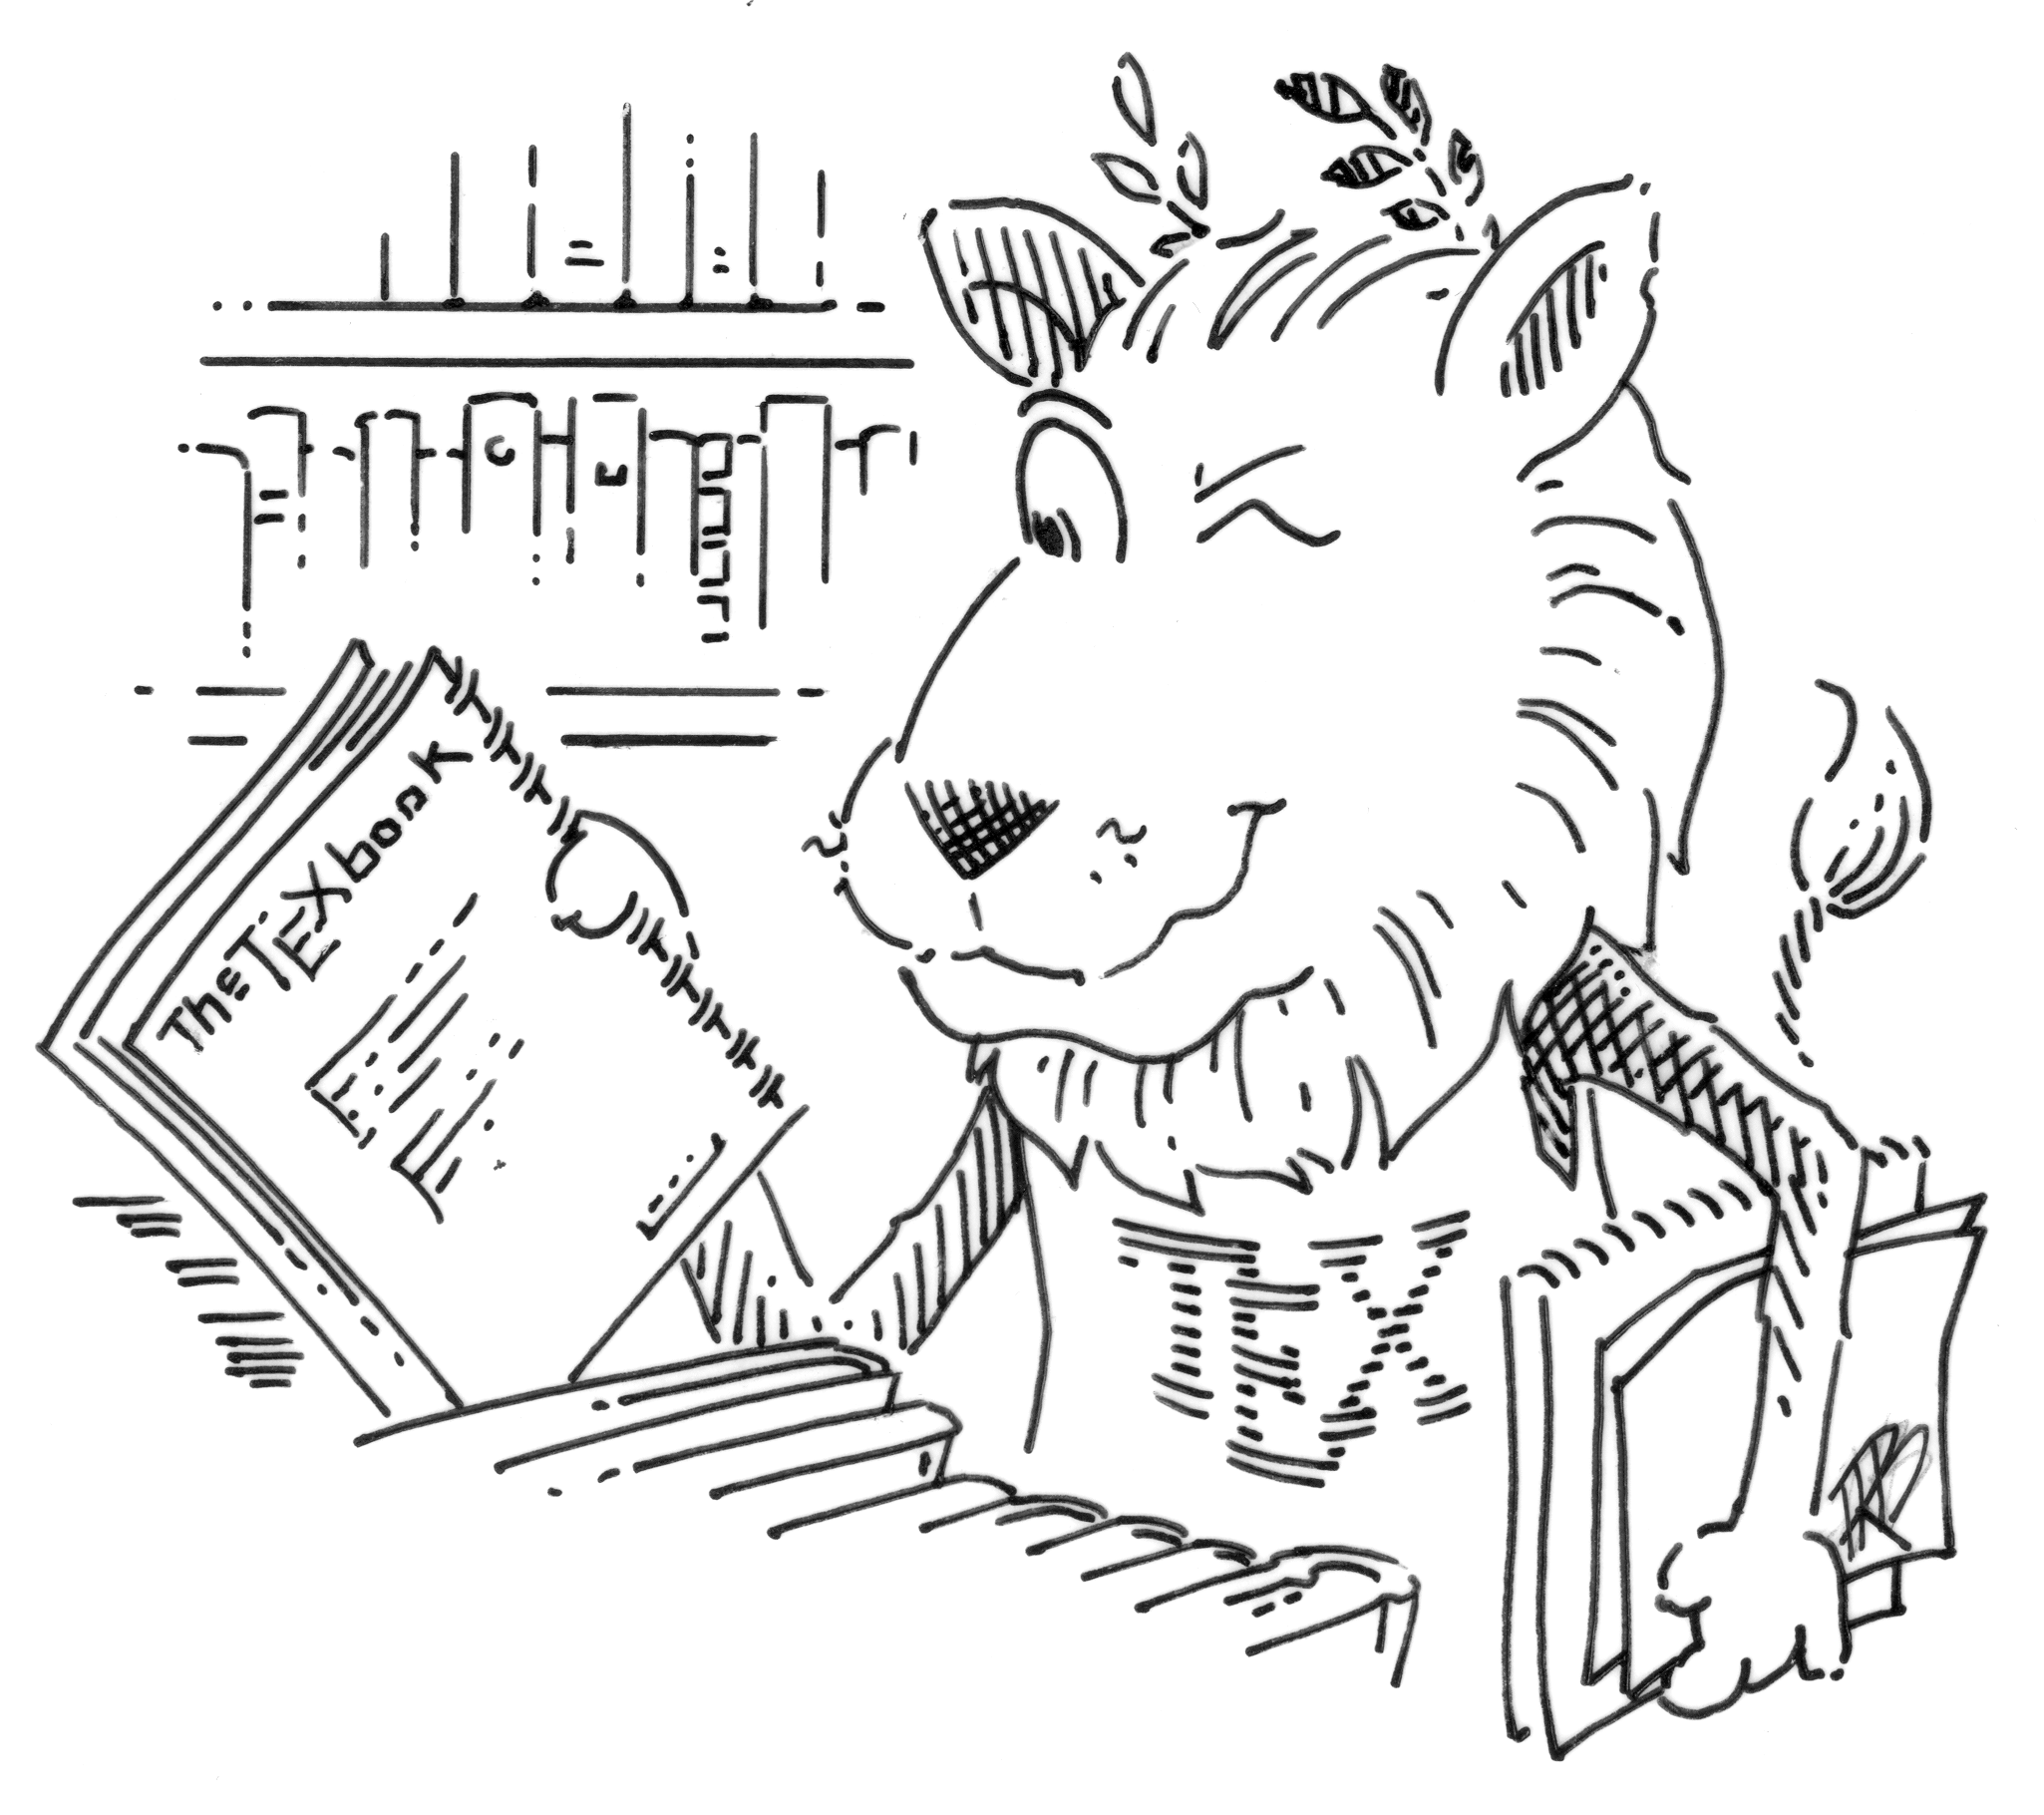
\includegraphics[width=0.8\linewidth]{tex_lion}
		\caption{El león Tex}
		\label{fig:leontex1}
	\end{wrapfigure}
	ggfdg gdfg gd gfdg gfgsgf ggsfg ggsdfg jhgjghjhk kjhgkhgkhg khgkhgkgh kjhkhkggkh khgkhgkh vxcvx cvxcv xcbcbvc bvcbv cbcvvnv nbmbn mnbmn bmn bmnb nbmnbmnb mn mnb mnbmbnmnb.
	
	
	ggfdg gdfg gd gfdg gfgsgf ggsfg ggsdfg jhgjghjhk kjhgkhgkhg khgkhgkgh kjhkhkggkh khgkhgkh vxcvx cvxcv xcbcbvc bvcbv cbcvvnv nbmbn mnbmn bmn bmnb nbmnbmnb mn mnb mnbmbnmnb.
	ggfdg gdfg gd gfdg gfgsgf ggsfg ggsdfg jhgjghjhk kjhgkhgkhg khgkhgkgh kjhkhkggkh khgkhgkh vxcvx cvxcv xcbcbvc bvcbv cbcvvnv nbmbn mnbmn bmn bmnb nbmnbmnb mn mnb mnbmbnmnb.
	ggfdg gdfg gd gfdg gfgsgf ggsfg ggsdfg jhgjghjhk kjhgkhgkhg khgkhgkgh kjhkhkggkh khgkhgkh vxcvx cvxcv xcbcbvc bvcbv cbcvvnv nbmbn mnbmn bmn bmnb nbmnbmnb mn mnb mnbmbnmnb.
	\begin{wrapfigure}[8]{r}{0.3\linewidth}
		\vspace{-5mm}
		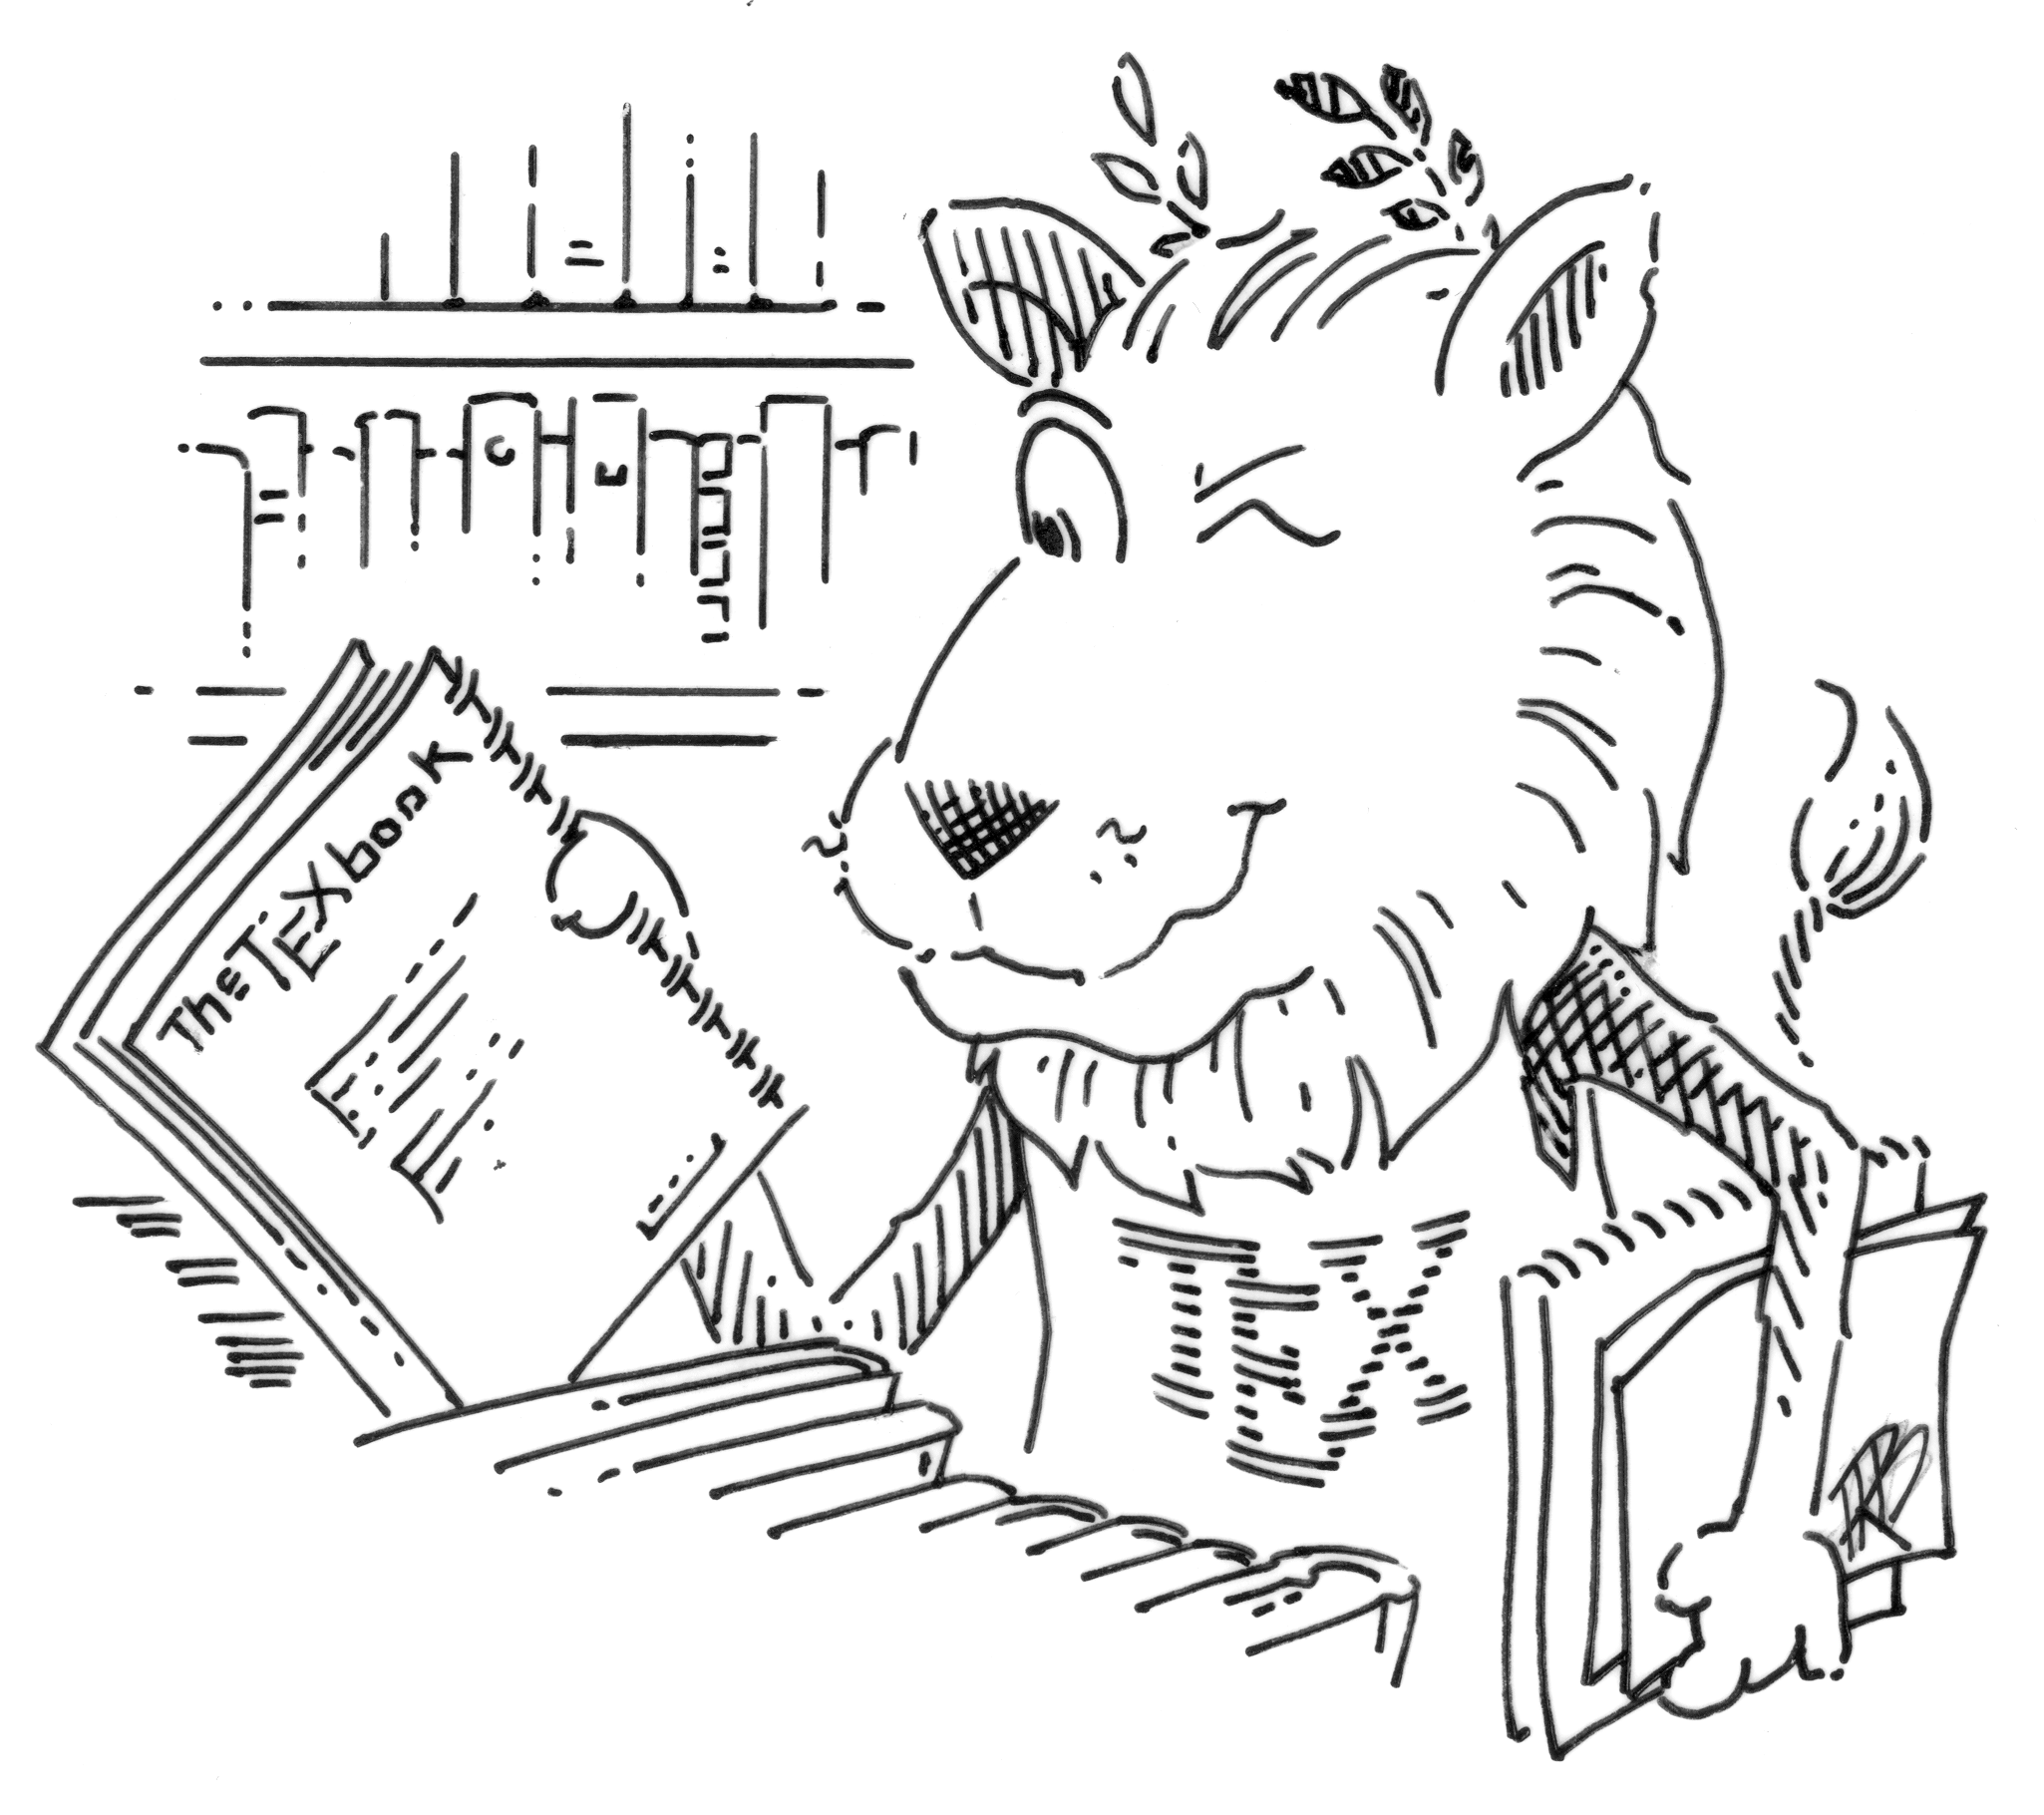
\includegraphics[width=0.8\linewidth]{tex_lion}
		\caption{El león Tex}
		\label{fig:leontex2}
	\end{wrapfigure}
	ggfdg gdfg gd gfdg gfgsgf ggsfg ggsdfg jhgjghjhk kjhgkhgkhg khgkhgkgh kjhkhkggkh khgkhgkh vxcvx cvxcv xcbcbvc bvcbv cbcvvnv nbmbn mnbmn bmn bmnb nbmnbmnb mn mnb mnbmbnmnb.
	ggfdg gdfg gd gfdg gfgsgf ggsfg ggsdfg jhgjghjhk kjhgkhgkhg khgkhgkgh kjhkhkggkh khgkhgkh vxcvx cvxcv xcbcbvc bvcbv cbcvvnv nbmbn mnbmn bmn bmnb nbmnbmnb mn mnb mnbmbnmnb.
	ggfdg gdfg gd gfdg gfgsgf ggsfg ggsdfg jhgjghjhk kjhgkhgkhg khgkhgkgh kjhkhkggkh khgkhgkh vxcvx cvxcv xcbcbvc bvcbv cbcvvnv nbmbn mnbmn bmn bmnb nbmnbmnb mn mnb mnbmbnmnb.
	
	ggfdg gdfg gd gfdg gfgsgf ggsfg ggsdfg jhgjghjhk kjhgkhgkhg khgkhgkgh kjhkhkggkh khgkhgkh vxcvx cvxcv xcbcbvc bvcbv cbcvvnv nbmbn mnbmn bmn bmnb nbmnbmnb mn mnb mnbmbnmnb.
	ggfdg gdfg gd gfdg gfgsgf ggsfg ggsdfg jhgjghjhk kjhgkhgkhg khgkhgkgh kjhkhkggkh khgkhgkh vxcvx cvxcv xcbcbvc bvcbv cbcvvnv nbmbn mnbmn bmn bmnb nbmnbmnb mn mnb mnbmbnmnb.
	
	\end{minipage}
	
	\clearpage
	\section{Texto sobre una figura}
	
	ggfdg gdfg gd gfdg gfgsgf ggsfg ggsdfg jhgjghjhk kjhgkhgkhg khgkhgkgh kjhkhkggkh khgkhgkh vxcvx cvxcv xcbcbvc bvcbv cbcvvnv nbmbn mnbmn bmn bmnb nbmnbmnb mn mnb mnbmbnmnb.
	ggfdg gdfg gd gfdg gfgsgf ggsfg ggsdfg jhgjghjhk kjhgkhgkhg khgkhgkgh kjhkhkggkh khgkhgkh vxcvx cvxcv xcbcbvc bvcbv cbcvvnv nbmbn mnbmn bmn bmnb nbmnbmnb mn mnb mnbmbnmnb.
	
	\begin{figure}[h]
		\color{colorGris1}\centering
		\begin{overpic}[width=0.6\linewidth, tics=5, grid]{plot}
			% Borrar grilla se quita el comando grid 
			\put (20,1) {5}
			\put (40,1) {10}
			\put (60,1) {15}
			\put (80,1) {20}
			\put (0,20) {5}
			\put (0,40) {10}
			\put (0,60) {15}
			\put (63,67) {Función f(x)}
		\end{overpic}
		\caption{Gráfico de una función}
		\label{fig:funcion1}
	\end{figure}
	
	ggfdg gdfg gd gfdg gfgsgf ggsfg ggsdfg jhgjghjhk kjhgkhgkhg khgkhgkgh kjhkhkggkh khgkhgkh vxcvx cvxcv xcbcbvc bvcbv cbcvvnv nbmbn mnbmn bmn bmnb nbmnbmnb mn mnb mnbmbnmnb.
	ggfdg gdfg gd gfdg gfgsgf ggsfg ggsdfg jhgjghjhk kjhgkhgkhg khgkhgkgh kjhkhkggkh khgkhgkh vxcvx cvxcv xcbcbvc bvcbv cbcvvnv nbmbn mnbmn bmn bmnb nbmnbmnb mn mnb mnbmbnmnb.
	ggfdg gdfg gd gfdg gfgsgf ggsfg ggsdfg jhgjghjhk kjhgkhgkhg khgkhgkgh kjhkhkggkh khgkhgkh vxcvx cvxcv xcbcbvc bvcbv cbcvvnv nbmbn mnbmn bmn bmnb nbmnbmnb mn mnb mnbmbnmnb.
	ggfdg gdfg gd gfdg gfgsgf ggsfg ggsdfg jhgjghjhk kjhgkhgkhg khgkhgkgh kjhkhkggkh khgkhgkh vxcvx cvxcv xcbcbvc bvcbv cbcvvnv nbmbn mnbmn bmn bmnb nbmnbmnb mn mnb mnbmbnmnb.
	
	\section{El entorno table}
	
	\begin{table}[h]
		\centering
		\caption{Ejemplo de tabla.}
		\begin{tabular}{|c|c|c|c|}
			\hline
			& 1 & 2 & 3 \\
			\hline
			A & & & \\
			\hline
			B & & & \\
			\hline
		\end{tabular}
		\label{tab:datos}
	\end{table}
	Esta es la referencia a la tabla \ref{tab:datos}
	
	\section{Personalizar tablas}
	
	ggfdg gdfg gd gfdg gfgsgf ggsfg ggsdfg jhgjghjhk kjhgkhgkhg khgkhgkgh kjhkhkggkh khgkhgkh vxcvx cvxcv xcbcbvc bvcbv cbcvvnv nbmbn mnbmn bmn bmnb nbmnbmnb mn mnb mnbmbnmnb.
	
	% Tabla sin personalizar
	\begin{table}[h]
		\centering
		\caption{Coeficientes parciales de seguridad en ELS.}
		\begin{tabular}{p{4cm}cc}
			\hline \textbf{Tipo de acción} & \textbf{Efecto desfavorable} & \textbf{Efecto favorable} \\
			\hline Permanente & gG=1 & gG=1 \\
			\hline Pretensado & 1.10 & 0.90 \\
			\hline Permanente de valor no constante & 1.00 & 1.00 \\
			\hline Variable &.00 & 0.00 \\
			\hline
		\end{tabular}
		\label{tab:coeficientes1}
	\end{table}
	
	Esta es la referencia a la tabla \ref{tab:datos}
	
	% Tabla sin personalizada
	\begin{table}[h]
		\centering
		\caption{Coeficientes parciales de seguridad en ELS.}
		\rowcolors{1}{white}{gray}
		\begin{tabular}{p{4cm}cc}
			\toprule % Primera línea
			\hline \textbf{Tipo de acción} & \textbf{Efecto desfavorable} & \textbf{Efecto favorable} \\
			\midrule % Segunda línea
			Permanente & gG=1 & gG=1 \\
			Pretensado & 1.10 & 0.90 \\
			Permanente de valor no constante & 1.00 & 1.00 \\
			Variable &.00 & 0.00 \\
			\bottomrule % Última línea
		\end{tabular}
		\label{tab:coeficientes2}
	\end{table}
	
	Esta es la referencia a la tabla \ref{tab:datos}
	
	
	sfsdafa sagdgdf ggfdg gdfg gd gfdg gfgsgf ggsfg ggsdfg jhgjghjhk kjhgkhgkhg khgkhgkgh kjhkhkggkh khgkhgkh vxcvx cvxcv xcbcbvc bvcbv cbcvvnv nbmbn mnbmn bmn bmnb nbmnbmnb mn mnb mnbmbnmnb.
	
	\section{Excel2LaTeX}
	
	ggfdg gdfg gd gfdg gfgsgf ggsfg ggsdfg jhgjghjhk kjhgkhgkhg khgkhgkgh kjhkhkggkh khgkhgkh vxcvx cvxcv xcbcbvc bvcbv cbcvvnv nbmbn mnbmn bmn bmnb nbmnbmnb mn mnb mnbmbnmnb.
	
	% Table generated by Excel2LaTeX from sheet 'Sheet1'
	\begin{table}[htbp]
		\centering
		\caption{Tablas de excel}
		\begin{tabular}{p{2.39em}p{15.28em}lllr}
			\multicolumn{1}{l}{} & \multicolumn{1}{r}{} & \multicolumn{4}{c}{\textbf{2021}} \\
			\midrule
			\textbf{Etapa} & \textbf{Productos/Entregables} & \multicolumn{1}{p{4.055em}}{\textbf{Ene-Mar}} & \multicolumn{1}{p{4.055em}}{\textbf{Abr-Jun}} & \multicolumn{1}{p{4.055em}}{\textbf{Jul-Set}} & \multicolumn{1}{p{4.055em}}{\textbf{Oct-Dic}} \\
			\midrule
			E1    & Primer documento a entregar, en .doc. &       & \cellcolor[rgb]{ .718,  .871,  .91} &       &  \\
			E2    & Segundo documento, más pesado. & \cellcolor[rgb]{ .776,  .89,  .859} &       &       &  \\
			E2    & Este tema mejor que no falte. &       & \cellcolor[rgb]{ .776,  .89,  .859} &       &  \\
			E2    & Otro tema interesante en PDF. &       &       & \cellcolor[rgb]{ .776,  .89,  .859} &  \\
			E2    & Esto es importante, también va. &       &       & \cellcolor[rgb]{ .776,  .89,  .859} &  \\
			E3    & Un documento para ver como vamos, editable. &       & \cellcolor[rgb]{ .722,  .804,  .894} &       &  \\
			E4    & Informe de evaluación hasta ahora. &       & \cellcolor[rgb]{ .722,  .804,  .894} &       &  \\
			E5    & Diseño final del sistema. &       &       &       & \cellcolor[rgb]{ .722,  .804,  .894} \\
			E6    & Recomendaciones estratégicas. &       &       &       & \cellcolor[rgb]{ .722,  .804,  .894} \\
			\bottomrule
		\end{tabular}%
		\label{tab:cronograma}%
	\end{table}%
		ggfdg gdfg gd gfdg gfgsgf ggsfg ggsdfg jhgjghjhk kjhgkhgkhg khgkhgkgh kjhkhkggkh khgkhgkh vxcvx cvxcv xcbcbvc bvcbv cbcvvnv nbmbn mnbmn bmn bmnb nbmnbmnb mn mnb mnbmbnmnb.
		
	Esta es la referencia a la \autoref{tab:cronograma} en la \autopageref{tab:cronograma}
	
\end{document}